%% REFERENCE DRAFT (written 31 Oct 2026 from the 29 Oct call with Jerome). Read draft.pdf, or set
%% Menu -> Main document -> draft.tex in Overleaf. The paper you write is main.tex; this file is not meant to be edited
%% into the final version.
%% Every number carries a "% src:" comment naming where it was read. Finished 7 Nov 2026: no [pending] mark is left; the
%% tables come from tools/paper_figs/make_paper_figures.py (figures/tab_*.tex). The body (up to the impact statement)
%% fits 8 pages in the ICML kit.
\documentclass{article}
%% Shared by main.tex (the paper you write) and draft.tex (the reference draft).
%% Format: the ICML 2026 kit, two columns, Times text and Computer Modern math. Page geometry, fonts and spacing
%% come from the kit and are never changed here. The kit is the provisional choice until the venue is decided:
%% for a journal (e.g. PRX Intelligence, revtex two-column), only this file and the \twocolumn[...] block in the
%% two main files change.

\usepackage{microtype}
\usepackage{graphicx}
\usepackage{booktabs}
\usepackage{xcolor}
\usepackage{hyperref}
\usepackage{tikz}
\usetikzlibrary{arrows.meta,calc,positioning}
\newcommand{\theHalgorithm}{\arabic{algorithm}}

% preprint: author names shown, footer "Preprint. <date>" (arXiv first, venue later).
% Anonymous submission: \usepackage{icml2026}.  Camera-ready: \usepackage[accepted]{icml2026}.
\usepackage[preprint]{icml2026}

\usepackage{amsmath}
\usepackage{amssymb}
\usepackage{mathtools}
\usepackage[capitalize,noabbrev]{cleveref}

\graphicspath{{figures/}}

%% ---------------------------------------------------------------- figures
%% Every plot is drawn at its printed size: 3.25 in for one column, 6.75 in for the full width (figure*).
%% Include them WITHOUT a width, so that the axis labels stay at the body's 10 pt:
%%     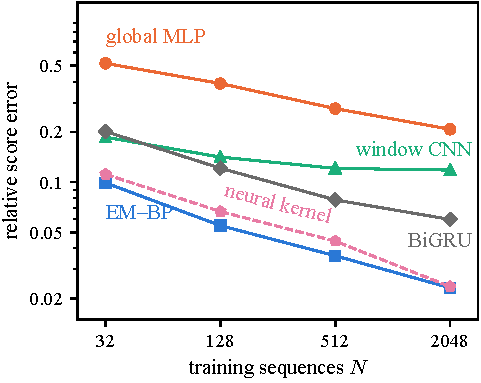
\includegraphics{fig_value_of_structure}
%% The plots and their style (box on all four sides, no grid, minor ticks, log scales, markers for measurements and
%% lines for closed forms) are made by tools/paper_figs/make_paper_figures.py in the research repository; see README.md.
%% The two diagrams are TikZ, \input from figures/*.tikz, so they use the body font and can be edited here.

%% ---------------------------------------------------------------- notation
\newcommand{\E}{\mathbb{E}}
\newcommand{\Normal}{\mathcal{N}}
\newcommand{\Kt}{K_\theta}
\newcommand{\dd}{\mathrm{d}}
\newcommand{\Dt}{\Delta_t}
\newcommand{\Ng}{N_g}

%% ---------------------------------------------------------------- writing aids
%% \note{...}    grey guidance text: what goes here, what Jerome asked for. Hide them all with \shownotesfalse.
%% \pending{...} a result that is not in yet (a run still on the cluster). Shown in orange so none is forgotten.
\newif\ifshownotes \shownotestrue
\definecolor{notegrey}{gray}{0.45}
\definecolor{pendingorange}{HTML}{C0501F}
\newcommand{\note}[1]{\ifshownotes{\color{notegrey}\itshape [#1]}\fi}
\newcommand{\pending}[1]{{\color{pendingorange}[pending: #1]}}


\icmltitlerunning{Learn the Kernel, Not the Score}

\begin{document}

\twocolumn[
\icmltitle{Learn the Kernel, Not the Score:\\ Belief-Propagation Denoisers for Markov Sequences}

\begin{icmlauthorlist}
  \icmlauthor{Giovanni Mantovani}{boc}
  \icmlauthor{J\'er\^ome Garnier-Brun}{boc}
  \icmlauthor{Marc M\'ezard}{boc}
\end{icmlauthorlist}
\icmlaffiliation{boc}{Department of Computing Sciences, Bocconi University, Milan, Italy}
\icmlcorrespondingauthor{Giovanni Mantovani}{giovanni-mantovani@studbocconi.it}
\icmlkeywords{diffusion models, belief propagation, expectation maximisation, Markov chains, denoising}
\vskip 0.3in
]

\printAffiliationsAndNotice{}

\begin{abstract}
A diffusion model is a denoiser trained at every noise level. When the data are first-order Markov sequences, such as
time series or one-dimensional physical fields, we ask what a denoiser gains from this structure and how it should use
it. The structure is not inherited by the score: for a Gaussian chain the precision matrix of the noisy data, tridiagonal
for clean data, fills in at intermediate noise. It survives in the posterior. A Markov chain observed through independent
noise is a tree, so belief propagation (BP) gives the exact posterior mean, and hence the exact score, at every noise
level once the transition kernel is known. Learning the denoiser thus reduces to learning a function of two variables,
which we do by expectation--maximisation with BP as the E-step, from noisy sequences alone and without differentiating
through BP. On a chain with Laplace innovations, kernels learned in this way give scores 2.1 to 2.8 times more accurate
than the best of six neural denoisers trained on the same data. A neural energy kernel, which assumes nothing beyond the
Markov property, matches the best hand-designed family and beats every network in at least 15 of 16 seeds at every
training-set size. On nine other chains, kernel families with a fixed innovation law fall to the error of a linear
denoiser once the chain leaves their class, while the neural kernel does not. The advantage shrinks as the data depart
from the Markov property, at a rate set by their distance to the closest first-order chain, and BP on pairs of sites
restores it for a second-order chain. On the stochastic Allen--Cahn field, the neural kernel, with at most 1{,}185
parameters, beats a diffusion U-Net with $1.2\times10^{7}$ parameters in 30 of 32 paired seeds at 2{,}048 training
sequences, and a five-parameter kernel with the form of the lattice action recovers the temperature to within one
percent.
% src: 2.1-2.8: reports/paper-figures/README.md (E02a em_bp vs E03 networks, paired, 16 seeds, N=32..2048)
% src: neural energy kernel: tools/core/read_e56.py (E56 frozen 1 Nov 2026): energy 0.0235 vs em_bp 0.0231 at N=2048;
%      paired wins against each of E03's six networks 16/16 at every N except BiGRU at N=512 (15/16)
% src: nine chains: figures/tab_chains.tex (tools/paper_figs/make_paper_figures.py::tab_chains on frozen E57 and E61)
% src: second-order chain: tools/core/read_e62.py (E62 frozen 6 Nov 2026)
% src: U-Net: E55 finished cells (frozen 7 Nov 2026, not yet read against the predictions), seeds 0-7, N=2048: energy below U-Net 8+8+8+6 of 32;
%      n_params em_energy 337 (1,185 at Theta=0.5), unet 11,774,977
% src: temperature: E33 (Theta-hat/Theta 0.9995-1.0068, answers note Q8)

\end{abstract}

\section{Introduction}
\label{sec:intro}

A diffusion model generates data by reversing a noising process, and the only object it has to learn is a denoiser:
for every noise level $t$, the best guess of the clean data $a$ given a noisy version $x$
\cite{sohl2015deep,ho2020denoising,song2021scorebased}. By Tweedie's formula the score that drives the reverse
process is an affine function of the posterior mean $\E[a\mid x]$ \cite{robbins1956empirical,efron2011tweedie}, so
learning the score and learning the denoiser are the same problem. Neural networks solve it from samples, at every
$t$ at once, and what they learn about the structure of the data is an active question
\cite{kadkhodaie2024generalization,kamb2024analytic,biroli2024dynamical}.

We study this question on data whose structure is known exactly: first-order Markov sequences. A Markov sequence is
fixed by its transition kernel $K(a_{k+1}\mid a_k)$. This covers a wide class of data with a direction or a
locality, from time series of causal processes to one-dimensional physical fields with nearest-neighbour interactions,
whose stationary law is a chain. The question is what a denoiser gains from knowing that the data are Markov, and how
it should use that knowledge.

The answer has three parts, which organise the paper.
First, the structure is \emph{not} in the score. For the Gaussian chain the score is linear and its matrix is
tridiagonal at $t=0$, but diffusion fills it in: at intermediate noise every site depends on every other
(\cref{sec:gaussian}). A denoiser constrained to be local, by a tridiagonal fit or a small receptive field, has an
error floor that no amount of data removes.
Second, the structure \emph{is} in the posterior. A Markov chain observed through independent noise is a tree, so
belief propagation (BP) computes $\E[a\mid x]$ exactly, for any kernel and at every $t$ (\cref{sec:tree}).
Third, learning the denoiser therefore reduces to learning the kernel. We do this by expectation--maximisation (EM),
with BP as the E-step, from noisy sequences only (\cref{sec:laplace}). BP enters the learning only through expected
transition counts, so the kernel can be any differentiable family, a small neural network included, without
differentiating through BP.

We test this on a non-Gaussian Markov chain with Laplace innovations, the simplest case where the exact score is not
linear, against six neural denoisers trained on the same data, and we measure how the comparison changes as the data
depart from the Markov property (\cref{sec:laplace}). We then apply it to the stochastic Allen--Cahn field, where the
choice of kernel family matters (\cref{sec:allen-cahn}).

\note{Related work in one paragraph here or in Sec.~7: HMM and Kalman EM \cite{baum1970,shumway1982em}; diffusion
from corrupted data with EM \cite{daras2023ambient,rozet2024learning,bai2024em}; BP and transformers on structured
data \cite{garnierbrun2024transformers}; analytic denoisers \cite{kamb2024analytic}. J\'er\^ome will help with the
literature.}

\section{Setting}
\label{sec:setting}

\paragraph{Data.} A clean sequence $a=(a_1,\dots,a_L)$ has one real number per site and is a first-order Markov
chain,
\begin{equation}
  p_0(a)=\mu(a_1)\prod_{k=1}^{L-1}K(a_{k+1}\mid a_k).
  \label{eq:chain}
\end{equation}
We take the chain stationary with unit variance, so the same kernel $K$ acts at every site. Nothing below needs this:
a site-dependent kernel changes the bookkeeping, not the method.

\paragraph{Noise and score.} We noise with the Ornstein--Uhlenbeck process, the variance-preserving diffusion of
\cite{song2021scorebased} at constant rate:
$x_k=e^{-t}a_k+\sqrt{\Dt}\,\xi_k$ with $\Dt=1-e^{-2t}$ and independent $\xi_k\sim\Normal(0,1)$. The score of the
noisy law is, by Tweedie's formula,
\begin{equation}
  S_t(x)_k=\nabla_{x_k}\log p_t(x)=\frac{e^{-t}\,\E[a_k\mid x]-x_k}{\Dt},
  \label{eq:tweedie}
\end{equation}
so a denoiser and a score model are the same object, and we compare methods by the score they produce.

\paragraph{Two chains.} The \emph{Gaussian chain} is $a_{k+1}=\alpha a_k+\sqrt{1-\alpha^2}\,\eta_k$ with Gaussian
$\eta_k$. The \emph{Laplace chain} has the same $\alpha$ and Laplace innovations of the same variance,
$\varepsilon_k\sim\mathrm{Laplace}(0,b)$ with $2b^2=1-\alpha^2$. The two have the same covariance, so every linear
denoiser treats them identically; any gain on the Laplace chain comes from its non-Gaussian structure alone. We use
$\alpha=0.85$ and $L=32$.

\paragraph{Error.} We report the relative score error
\begin{equation}
  e=\Big(\sum\lVert \hat S_t(x)-S_t^\star(x)\rVert^2\Big/\sum\lVert S_t^\star(x)\rVert^2\Big)^{1/2},
  \label{eq:error}
\end{equation}
where the sums run over test sequences, sites and twelve noise levels log-spaced from $t=0.05$ to $t=3$, and
$S^\star_t$ is the exact score. The error is $0$ for the exact score and $1$ for the zero estimate.

\section{The Gaussian chain: diffusion breaks locality}
\label{sec:gaussian}

\begin{figure*}[t]
  \centering
  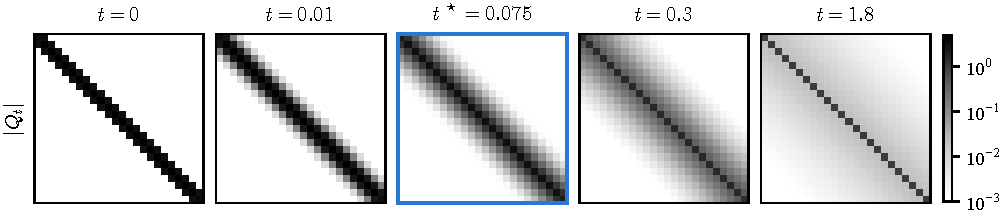
\includegraphics{fig_locality}
  \caption{Diffusion makes the score non-local. Magnitude of the score matrix $Q_t$ of the Gaussian chain
  ($\alpha=0.85$, $L=24$) at five noise levels, log colour scale. At $t=0$ it is the tridiagonal precision of the
  chain; at large $t$ it tends to the identity; in between, at $t^\star\simeq0.075$ (framed), the coupling beyond
  nearest neighbours is largest.}
  \label{fig:locality}
  % src: closed form, tools/paper_figs/make_paper_figures.py::fig_locality (t* = 0.0753 printed by the generator)
\end{figure*}

For the Gaussian chain everything is linear. The noisy data are Gaussian with covariance
$\Sigma_t=e^{-2t}\Sigma_0+\Dt\,I$, and the score is $S_t(x)=-Q_tx$ with $Q_t=\Sigma_t^{-1}$. At $t=0$ the matrix
$Q_0=\Sigma_0^{-1}$ is tridiagonal: this is the Markov property, written as a statement about the score. Each site
only talks to its two neighbours.

Diffusion does not preserve this. $\Sigma_t$ is a dense matrix plus a diagonal, and its inverse is not banded
(\cref{fig:locality}). The coupling of site $k$ to site $k+r$ decays geometrically in $r$, with a rate that depends on
$t$, and the matrix is furthest from tridiagonal at an intermediate level $t^\star\simeq0.075$ for $\alpha=0.85$
(\cref{app:numerics}). At large $t$ the noise dominates and $Q_t$ approaches the identity.
% src: t* = 0.0753, fig_locality / fig_locality_curve

The consequence is that locality cannot be obtained by constraining the denoiser. A denoiser that only sees a window
of radius $r$ around each site has an error floor even with unlimited data. For the Gaussian chain this floor is a
closed form: the best radius-$r$ estimator has relative score error $0.20$ for $r=1$, the nearest neighbours a
tridiagonal fit would use, $0.089$ for $r=2$, and still $0.029$ for $r=4$.
% src: thesis tools/fig_ch10.py::windowed_oracle([1,2,4,8]) = 0.2023, 0.0890, 0.0294, 0.0066 (alpha=0.85, L=32, 12 levels)
The structure has to be imposed elsewhere.

It is imposed on the model of the data. The posterior $p(a\mid x)$ is proportional to
$p_0(a)\prod_k\ell_t(x_k\mid a_k)$, with $\ell_t(x_k\mid a_k)=\Normal(x_k;e^{-t}a_k,\Dt)$, and is again a chain: the
noise is independent from site to site, so it adds one factor per site and no new link. For the Gaussian chain,
inference on this chain is the Kalman smoother \cite{kalman1960new,rauch1965maximum}, which returns $-Q_tx$ exactly
in $O(L)$ operations without ever forming $Q_t$. The next section does the same for any kernel.

\section{A noisy Markov chain is a tree}
\label{sec:tree}

\begin{figure}[t]
  \centering
  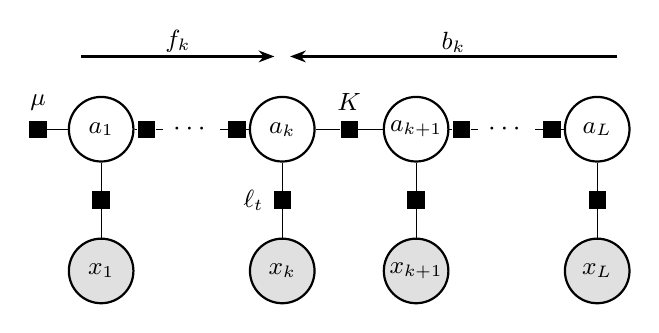
\begin{tikzpicture}[
    var/.style={circle,draw,thick,minimum size=8.2mm,inner sep=0pt,font=\small},
    obs/.style={circle,draw,thick,fill=black!12,minimum size=8.2mm,inner sep=0pt,font=\small},
    fac/.style={rectangle,fill=black,minimum size=2.2mm,inner sep=0pt},
    lab/.style={font=\small,inner sep=1pt},
    msg/.style={-{Stealth[length=2mm]},thick}]
  \node[var] (a1) at (0,0) {$a_1$};
  \node (d1) at (1.15,0) {$\cdots$};
  \node[var] (ak) at (2.3,0) {$a_k$};
  \node[var] (ak1) at (4.0,0) {$a_{k+1}$};
  \node (d2) at (5.15,0) {$\cdots$};
  \node[var] (aL) at (6.3,0) {$a_L$};
  \node[fac] (m0) at (-0.8,0) {};
  \draw (m0) -- (a1);
  \node[lab,above=0.8mm of m0] {$\mu$};
  \foreach \u/\v/\n in {a1/d1/ka,d1/ak/kb,ak/ak1/kc,ak1/d2/kd,d2/aL/ke} {
    \node[fac] (\n) at ($(\u)!0.5!(\v)$) {};
    \draw (\u) -- (\n) -- (\v);
  }
  \node[lab,above=0.8mm of kc] {$K$};
  \foreach \i/\n in {a1/1,ak/k,ak1/{k+1},aL/L} {
    \node[fac] (o\i) at ($(\i)+(0,-0.9)$) {};
    \node[obs] (x\i) at ($(\i)+(0,-1.8)$) {$x_{\n}$};
    \draw (\i) -- (o\i) -- (x\i);
  }
  \node[lab,left=0.8mm of oak] {$\ell_t$};
  \draw[msg] ($(a1.north)+(-0.25,0.5)$) -- node[lab,above]{$f_k$} ($(ak.north)+(-0.1,0.5)$);
  \draw[msg] ($(aL.north)+(0.25,0.5)$) -- node[lab,above]{$b_k$} ($(ak.north)+(0.1,0.5)$);
\end{tikzpicture}

  \caption{Factor graph of the posterior $p_t(\mathbf a\mid\mathbf x)$ of \cref{eq:posterior_chain}. White circles are
  the clean values $a_k$, grey circles the noisy observations $x_k$, which are known. Black squares are the factors: the
  law $\mu$ of the first site, the kernel $K(a_{k+1}\mid a_k)$ between neighbours and the noise term
  $\ell_t(x_k\mid a_k)$ at each site. There is no loop, so belief propagation is exact. The forward message $f_k$ carries
  what $x_1,\ldots,x_k$ say about $a_k$, the backward message $b_k$ what $x_{k+1},\ldots,x_L$ say about it, and the
  posterior of $a_k$ is proportional to $f_k(a_k)\,b_k(a_k)$.}
  \label{fig:factor-graph}
\end{figure}

\paragraph{Beyond Gaussianity.}
The Gaussian chain is exactly solvable and linear. We now take a controlled non-Gaussian step, the Laplace chain
\begin{equation}
    a_{k+1}=\alpha a_k+\varepsilon_k,
    \qquad
    \varepsilon_k\sim\operatorname{Laplace}(0,b),
    \label{eq:laplace_chain}
\end{equation}
with $2b^2=1-\alpha^2$. The noise has the same variance as in the Gaussian chain, so the two chains have the same
covariance. But the Laplace noise has a sharp peak and heavier tails, and the score is no longer linear in $\mathbf x$.

\paragraph{The posterior factor graph.}
The first-order Markov structure survives the noise. Combining the kernel with the independent noise terms gives
\cref{eq:posterior_chain}, whose factor graph is a chain with one extra factor on each site (\cref{fig:factor-graph}).
Since the noise acts on each site separately, conditioning on the observations adds no edge. The posterior is still
connected and has no loop: it is a tree, where the cavity method and belief propagation are exact
\cite{mezard2001bethe,mezard2006reconstruction,mezard2009information}.

\paragraph{Exact inference by belief propagation.}
On a tree, the sum--product algorithm gives the exact marginals with one forward and one backward pass
\cite{pearl1988probabilistic,kschischang2001factor,yedidia2003understanding}. With forward messages $f_k$ and backward
messages $b_k$, the recursions are
\begin{align}
    f_1(a_1)
    &=\mu(a_1)\ell_t(x_1\mid a_1),\nonumber\\
    f_{k+1}(a_{k+1})
    &=\ell_t(x_{k+1}\mid a_{k+1})\nonumber\\
    &\qquad\times\int K(a_{k+1}\mid a_k)f_k(a_k)\,da_k,\nonumber\\
    b_L(a_L)&=1,\nonumber\\
    b_k(a_k)
    &=\int K(a_{k+1}\mid a_k)
      \ell_t(x_{k+1}\mid a_{k+1})\nonumber\\
    &\qquad\times b_{k+1}(a_{k+1})\,da_{k+1}.
    \label{eq:bp}
\end{align}
The posterior of one site is then
\begin{equation}
    p(a_k\mid\mathbf x)
    \propto f_k(a_k)b_k(a_k),
\end{equation}
and its mean gives the score through \cref{eq:tweedie}:
\begin{equation}
    S_{t,k}(\mathbf x)=\frac{e^{-t}}{\Delta_t}\,
    \frac{\int a\,f_k(a)b_k(a)\,da}{\int f_k(a)b_k(a)\,da}-\frac{x_k}{\Delta_t}.
\end{equation}

So, for any known first-order kernel, two sweeps of messages give the exact joint score, with no assumption of
Gaussianity or linearity. The noise level only enters through $\ell_t$, so one kernel gives the score at every $t$.
The same exact inference on a tree is at the heart of the hierarchical models of \cite{garnierbrun2024transformers},
where transformers trained on such data learn to approximate BP; a Markov chain is the simplest tree.

\section{Learning the kernel: the Laplace chain}
\label{sec:laplace}

In practice the kernel is unknown and only data are available. This section learns it from noisy sequences, on the
Laplace chain, where the exact score is known and is not linear.

\subsection{Expectation--maximisation through BP}
\label{sec:em}

\begin{figure}[t]
  \centering
  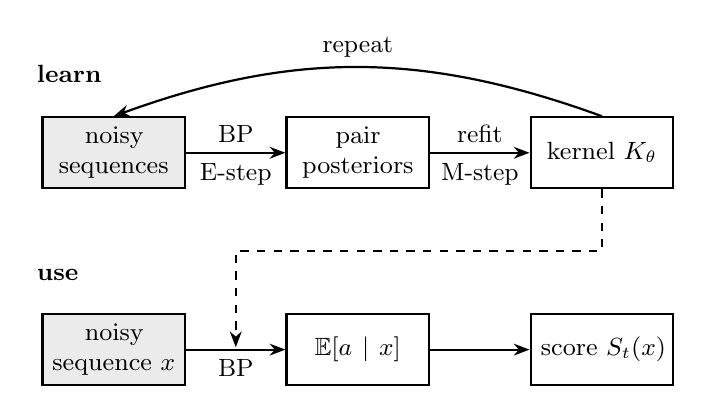
\begin{tikzpicture}[
    box/.style={draw,thick,align=center,font=\small,minimum height=9mm,inner sep=3pt,text width=1.6cm},
    data/.style={box,fill=black!8},
    arr/.style={-{Stealth[length=2mm]},thick},
    lab/.style={font=\small,align=center}]
  \node[font=\small\bfseries,anchor=west] at (-1.1,1.0) {learn};
  \node[data] (d) at (0,0) {noisy\\ sequences};
  \node[box] (p) at (3.1,0) {pair\\ posteriors};
  \node[box] (k) at (6.2,0) {kernel $K_\theta$};
  \draw[arr] (d) -- node[above,lab]{BP} node[below,lab]{E-step} (p);
  \draw[arr] (p) -- node[above,lab]{refit} node[below,lab]{M-step} (k);
  \draw[arr] (k.north) to[out=160,in=20] node[above,lab]{repeat} (d.north);
  \node[font=\small\bfseries,anchor=west] at (-1.1,-1.55) {use};
  \node[data] (x) at (0,-2.5) {noisy\\ sequence $x$};
  \node[box] (m) at (3.1,-2.5) {$\mathbb{E}[a\mid x]$};
  \node[box] (s) at (6.2,-2.5) {score $S_t(x)$};
  \draw[arr] (x) -- node[below,lab]{BP} (m);
  \draw[arr] (m) -- (s);
  \draw[thick,dashed,-{Stealth[length=2mm]}] (k.south) -- (6.2,-1.25) -| (1.55,-2.47);
\end{tikzpicture}

  \caption{Learning and using the kernel. Learn: BP with the current kernel gives the posterior of every pair of
  neighbouring sites (E-step); the kernel is refitted to these pairs (M-step); repeat. Use: BP with the learned
  kernel gives $\E[a\mid x]$, hence the score, at any noise level.}
  \label{fig:em-loop}
\end{figure}

Let $\Kt$ be a parametric family of kernels and $x^{(1)},\dots,x^{(N)}$ noisy training sequences, each at its own
noise level. The likelihood $p_\theta(x)$ sums over all clean sequences compatible with $x$, and BP computes it: it is
the product of the normalisers of the forward messages. Maximising it directly is possible but unnecessary. EM
\cite{dempster1977maximum} splits the problem into the two steps of \cref{fig:em-loop}.

The E-step runs BP with the current parameters $\theta_{\rm old}$ and collects, for every link $k$, the posterior of
the pair,
\begin{align}
  \xi_k(a,a')&=p_{\theta_{\rm old}}(a_k=a,\,a_{k+1}=a'\mid x)\nonumber\\
  &\propto\mu_{\to}^{k}(a)\,K(a'\mid a)\,\ell_t(x_{k+1}\mid a')\,\mu_{\leftarrow}^{k+1}(a').
\end{align}
Summed over links and sequences, $\Xi(a,a')=\sum_{d,k}\xi_k^{(d)}(a,a')$ is the expected number of transitions from
$a$ to $a'$ in the clean data, given what the noisy data show. The M-step then raises
\begin{equation}
  Q(\theta)=\iint\Xi(a,a')\,\log\Kt(a'\mid a)\,\dd a\,\dd a',
  \label{eq:Q}
\end{equation}
the expected log-likelihood of the clean data under the current posterior. With clean data $\Xi$ is the histogram of
observed transitions and the M-step is ordinary maximum likelihood; with noisy data the counts are soft.

The logic is that of following the gradient of an expectation. BP gives the expectation; $\Kt$ is a controlled
function of $\theta$; and the gradient of $Q$ at $\theta_{\rm old}$ is exactly the gradient of the log-likelihood,
$\nabla_\theta\log p_\theta(x)=\nabla_\theta Q(\theta)\rvert_{\theta=\theta_{\rm old}}$ (Fisher's identity,
\cite{louis1982,cappe2005}). Each M-step therefore moves uphill on the likelihood, and the likelihood never decreases
\cite{wu1983}. Two practical consequences follow. First, BP enters the M-step only through $\Xi$, which is fixed
while $\theta$ moves: the gradient of $Q$ goes through $\Kt$ and its normalisation on the grid, never through BP. Any
differentiable family can be trained with ordinary automatic differentiation, a neural network included. Second,
the noise level appears only in the E-step, so the kernel is learned once for all $t$ and no noise schedule is
needed for training.

\subsection{Kernel families}
\label{sec:families}

\begin{figure*}[t]
  \centering
  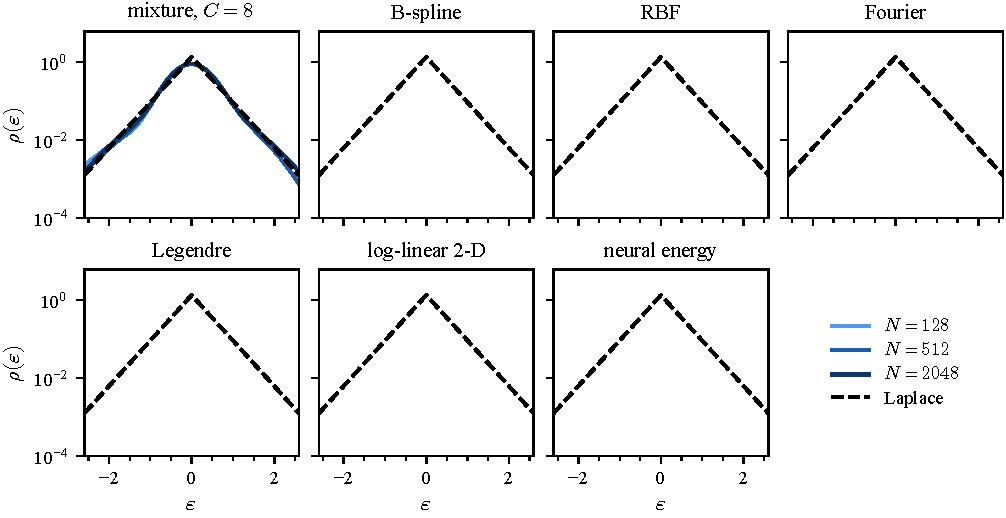
\includegraphics{fig_families}
  \caption{What each kernel family learns. Learned law of the innovation $\varepsilon=a_{k+1}-\alpha a_k$ (for the two
  agnostic families, the learned $K(\varepsilon\mid a=0)$) from $N=128$, $512$ and $2048$ noisy sequences, against the
  Laplace truth (dashed). One seed per $N$. \pending{E56 fits for all panels but the mixture; mixture from exp\_18.}}
  \label{fig:families}
\end{figure*}

\Cref{fig:families} shows what different families learn.
A first choice is a mixture of $C=8$ Gaussians for the innovation,
$\Kt(a'\mid a)=\sum_c\pi_c\Normal(a'-\alpha a;\nu_c,s_c^2)$, with 25 parameters and an almost closed-form M-step. It
learns the coefficient $\alpha$ to within $0.1\%$ from $N=512$ sequences, but it can only approximate the kink by
stacking Gaussians, and the excess kurtosis of its innovation stays $6$ to $25\%$ off (\cref{app:em}).
% src: reports/paper-figures/README.md, fig_em_innovation (exp_18): alpha within 0.1% from N=512 (2.4% at 128); kurtosis 6-25%
Nothing makes a mixture of Gaussians the natural choice. We therefore also expand $\log\Kt$, not $\Kt$, in a basis:
the innovation law is $\phi(\varepsilon)\propto\exp\big(-\lambda\varepsilon^2/2+\sum_mc_m\,b_m(\varepsilon)\big)$ with
$b_m$ cubic B-splines, Gaussian radial basis functions, a truncated Fourier series, or Legendre polynomials, 25
parameters each. Putting the expansion on $\log\Kt$ keeps the kernel positive and makes $Q$ concave in the
coefficients, so every M-step has a unique maximum. Local bases (splines, radial functions) can bend sharply at one
point; global ones (Fourier, Legendre) can only approximate a kink by oscillating.

These are all \emph{shift} families: they assume $a_{k+1}=\alpha a_k+\varepsilon_k$ with $\varepsilon_k$ independent
of $a_k$. Two further families assume nothing. A log-linear kernel expands $\log\Kt(a'\mid a)$ in a tensor B-spline
basis of both arguments (100 parameters). A neural energy kernel sets $\Kt(a'\mid a)\propto\exp(-E_\theta(a,a'))$
with $E_\theta$ a multilayer perceptron with two hidden layers; normalised on the grid, it can represent any smooth
kernel, and it is trained by the same M-step, with a few gradient steps on $Q$ per iteration.
\pending{E56: which family recovers the kink, and at which $N$.}

\subsection{Against neural denoisers}
\label{sec:networks}

\begin{figure}[t]
  \centering
  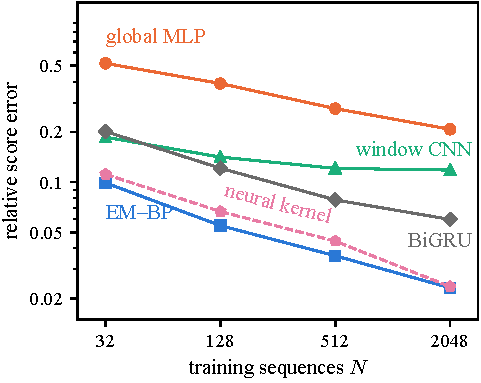
\includegraphics{fig_value_of_structure}
  \caption{Relative score error against the number of training sequences, on the same test sequences. EM--BP with
  the mixture kernel; a global MLP (no locality); a window CNN (locality); BiGRU, the best of six architectures from
  $N=128$ up. Mean over 16 seeds.}
  \label{fig:value-of-structure}
  % src: outputs/E02a/capacity.csv (em_bp, C=8) + outputs/E03/confirm.csv, paired on test bundles (384 of 384 rows)
\end{figure}

\begin{figure}[t]
  \centering
  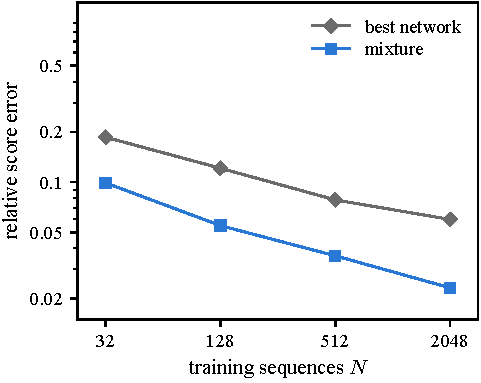
\includegraphics{fig_families_error}
  \caption{Relative score error of every kernel family against $N$, with the best of six networks at each $N$ for
  reference. Same test sequences as \cref{fig:value-of-structure}. \pending{E56.}}
  \label{fig:families-error}
\end{figure}

We compare the learned kernel with neural denoisers trained by denoising score matching \cite{vincent2011connection}:
a global MLP, which has no notion of locality, a window CNN, which has it, and four standard sequence models (BiGRU,
TCN, transformer and U-Net). Each architecture's hyperparameters were screened on separate development seeds and its
checkpoint chosen on a validation set. The networks are trained on the clean training sequences with fresh noise at
every step. EM sees one noisy copy of each sequence, at one noise level, which is a disadvantage for EM.
\note{Appendix D: architectures, parameter counts (MLP 26{,}016, CNN 5{,}505, BiGRU 15{,}169), training recipe.}

\Cref{fig:value-of-structure} puts the three types of model on one plot. With 25 parameters, EM--BP has the lowest
error at every $N$, from $0.099$ at $N=32$ to $0.023$ at $N=2048$.
% src: seed means em_bp 0.0989, 0.0548, 0.0361, 0.0231 (N=32..2048), _paired_e03
The global MLP is $5.8$ to $9.9$ times worse and the window CNN $2.1$ to $5.6$ times worse. The CNN's error barely
improves with $N$ (from $0.14$ at $N=128$ to $0.12$ at $N=2048$), as the window floor of \cref{sec:gaussian}
leads one to expect. The best network at each $N$ is $2.1$ to $2.8$ times worse than EM--BP: the window CNN at $N=32$,
BiGRU above.
% src: mean per-seed ratios, reports/paper-figures/README.md: MLP 5.79/7.95/7.88/9.85, CNN 2.07/2.87/3.45/5.58, BiGRU 2.22/2.45/2.24/2.83
% src: window CNN seed means 0.1861, 0.1413, 0.1209, 0.1181
Both sides here select with the exact score of the validation sequences. Selecting instead by the likelihood of the
noisy validation sequences (EM) and the validation denoising loss (networks) changes the errors by at most $7\%$, and
the kernels stay below the best network in at least 15 of 16 seeds at every $N$ (\cref{app:em}).
% src: tools/core/read_e65.py on outputs/hpc_E65_{k_h0,k_h8,nets} (E65, frozen 4 Nov 2026, 976b595): free/oracle max
% em_bp 1.7%, spline 6.9%, energy 6.9%, networks <= 3.4% (BiGRU); paired below best network 16/16, 16/16, >= 15/16.
% E65's registered P3 is VOID (TCN and transformer missed the 2% reproduction gate): this sentence is descriptive.
\Cref{fig:families-error} adds the other kernel families. \pending{E56: does the neural energy kernel beat the
networks at small $N$, as the registered prediction says.}

\paragraph{The model or the objective?} Trained with the networks' own objective and data, denoising score matching
on the clean sequences with the score computed by a differentiable BP (\cref{app:networks}), the neural energy kernel
is still below the best network in 16 of 16 seeds at every $N$ ($0.018$ against BiGRU's $0.060$ at $N=2048$): the gain
comes from the model. The objective matters too: maximum likelihood on the same sequences is $1.3$ to $2.5$ times more
accurate still.
% src: tools/core/read_e66.py (E66, frozen 4 Nov 2026, 976b595): bp_dsm 0.0557/0.0329/0.0236/0.0183, BiGRU 0.0596 at
% N=2048, P1 16/16 at every N; bp_dsm / E58 energy_h16 (clean ML) = 1.33, 1.31, 1.82, 2.46 at N = 32..2048 (P2 FALSIFIED).

\subsection{Step efficiency}
\label{sec:steps}

\begin{figure*}[t]
  \centering
  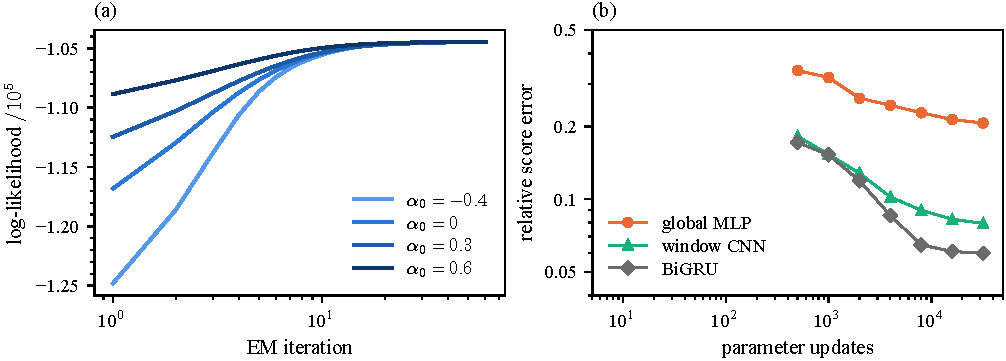
\includegraphics{fig_em_dynamics}
  \caption{Training dynamics. (a) Log-likelihood of the training data against EM iteration, from four starting
  values $\alpha_0$ of the coefficient (mixture kernel, $C=8$). (b) Validation score error against the number of
  parameter updates, $N=2048$: EM iterations for EM--BP, SGD steps for the networks, mean over 16 seeds.
  \pending{E56 EM--BP curve in (b); (a) then from E56, per transition.}}
  \label{fig:em-dynamics}
  % src: (a) Diffusion/research/nongaussian-bp/outputs/frozen/exp_18/em_trace.csv; (b) outputs/E03/confirm.csv val_curve
\end{figure*}

EM needs far fewer parameter updates than gradient training. From every starting point the likelihood rises
monotonically and reaches the same plateau within about twenty iterations (\cref{fig:em-dynamics}a). Parameters that
the likelihood constrains only weakly take longer: over 16 seeds, $\alpha$ settles in a median of 80 updates and the
shape of the innovation law in 229 (at most 638).
% src: memory em-shape-convergence (thesis exp_27, 16 seeds, C=8): rho median 80, shape 229, tail 638
The networks are still improving after $3.2\times10^4$ SGD steps (\cref{fig:em-dynamics}b).

Fewer updates do not mean less time: an EM iteration, a BP pass over all the data, costs 190 to 270 BiGRU steps at
$N=2048$ (\cref{app:compute}). From noisy data the energy kernel reaches the error of BiGRU's selected checkpoint first
in only 7 of 16 seeds at $N=2048$, and its own selected checkpoint later than BiGRU in all 16; from clean data, where an
M-step is one maximum-likelihood fit, it is first in 16 of 16 seeds at every $N\geq128$. At test time BP costs 6 to
20 times a sequence model's forward pass.
% src: tools/core/read_e63.py on outputs/hpc_E63 + E65's curves (E63, frozen 4 Nov 2026, 976b595): s per update at
% N=2048 em_bp 3.40, spline 2.34, energy 2.49, clean_energy 0.482, BiGRU 0.0126 (271x, 187x, 198x); P1 FALSIFIED 7/16,
% P3 16/16, P2 16/16 at N=128/512/2048; use time BP 6972 us vs TCN 1219, transformer 952, U-Net 904, BiGRU 343 us.
% NOTE: the exp_27 figures ("80", "229", "638") come from the memory file, not from a reader script; re-read before submission.

\subsection{Generation}
\label{sec:generation}

With the same ancestral sampler for every model (400 steps down to $t=0.005$; the networks retrained on continuous
levels, \cref{app:generation}), the kernels' samples are closer to the chain. At $N=2048$ the sliced Wasserstein
distance to exact samples is $0.059$ for EM--BP against $0.109$ for BiGRU, the best network, and $0.053$ between two
exact samples. At $N=128$ the clean-data kernel is below every network in at least 7 of 8 seeds, and its residuals'
excess kurtosis is closer to the Laplace value than the best network's in 6 of 8 seeds at both $N$. The samples'
likelihood under the true chain does not rank the models: with the true kernel the sampler scores worse on it than the
window CNN (\cref{app:generation}).
% src: tools/core/read_e64.py on outputs/hpc_E64 (E64, frozen 4 Nov 2026, 976b595), seed means over 8 seeds: SW2 at
% N=2048 em_bp 0.0590, clean_energy 0.0597, bigru_cont 0.1087, exact 0.0532; N=128 clean_energy 0.0966, best net
% window_cont 0.1327; P2 (7/8 at N=128, 8/8 at N=2048), P3 (6/8) CONFIRMED; |loglik gap| oracle_sampler 1.398,
% window_cont 0.373 at N=2048, P4 FALSIFIED.

\subsection{When the data are not Markov}
\label{sec:nonmarkov}

\begin{figure}[t]
  \centering
  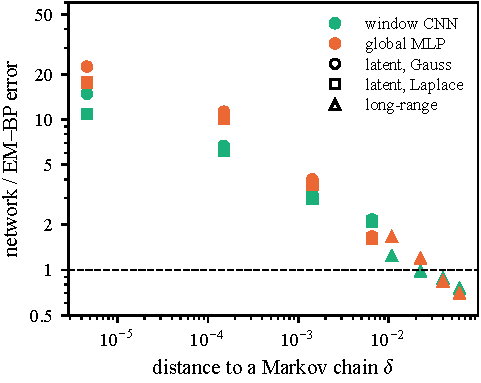
\includegraphics{fig_nonmarkov}
  \caption{Error of a network over that of EM--BP when the data are not Markov, against $\delta$, the distance per
  site from the data to the closest first-order chain. Global latent variable on the Gaussian and the Laplace chain,
  and long-range couplings on the Gaussian chain, each at four strengths. Below the dashed line the network wins.}
  \label{fig:nonmarkov}
  % src: thesis tools/fig_ch10.py::_nonmarkov (frozen exp_21_clean), delta closed form (kl_per_site)
\end{figure}

EM--BP assumes a first-order chain. To see how far this assumption can be wrong, we break it in two ways. A global
latent variable adds one Gaussian draw $g$ per sequence to every site, $a=(y+\beta g)/\sqrt{1+\beta^2}$ with $y$ a
Markov chain; long-range couplings add to the precision of the Gaussian chain a term $\gamma Q_{\rm long}$ that
couples distant sites. Both are measured by the same number, the Kullback--Leibler divergence per site from the
data's covariance to that of the closest first-order chain, $\delta$, in closed form.

\Cref{fig:nonmarkov} shows that both mechanisms, and both chains, fall on one curve. Close to Markov, at
$\delta\approx5\times10^{-6}$, the CNN is $11$ to $15$ times worse than EM--BP and the MLP $18$ to $22$ times.
The advantage shrinks steadily as $\delta$ grows, and the network wins beyond $\delta^\star\approx1$--$2\times10^{-2}$
nats per site for the CNN and $2$--$4\times10^{-2}$ for the MLP.
% src: generator printout: beta=0.1 d=4.61e-6 cnn 14.84/10.92 mlp 22.48/17.64; long-range cnn 1.24 -> 0.97 between d=1.08e-2 and 2.24e-2; mlp 1.19 -> 0.84 between 2.24e-2 and 3.96e-2
Part of the global latent is absorbed into the learned kernel: at $\beta=1$ the learned coefficient moves from $0.848$
to $0.939$, close to that of the best first-order chain.
% src: answers note Q12 (thesis Sec. 8.6, Table 8.9)
\pending{second-order chain $a_k=\phi_1a_{k-1}+\phi_2a_{k-2}+\varepsilon_k$, with EM--BP on the pair state
$(a_{k-1},a_k)$ as the repair.}

\section{Application: the stochastic Allen--Cahn field}
\label{sec:allen-cahn}

\begin{figure*}[t]
  \centering
  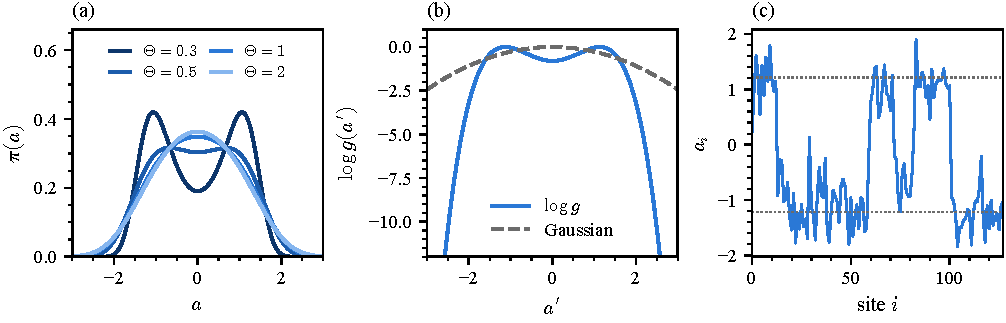
\includegraphics{fig_field}
  \caption{The Allen--Cahn chain. (a) Single-site law of the standardised field at the four temperatures.
  (b) The tilt $\log g$ of the kernel at $\Theta=0.3$ against the quadratic of the Gaussian chain with the same
  correlation. (c) One exact sample at $\Theta=0.3$; dotted lines mark the two wells.}
  \label{fig:field}
\end{figure*}

The stochastic Allen--Cahn equation\note{cite} describes a scalar field relaxing in a double-well potential,
\begin{equation}
  \partial_\tau\phi=\partial_x^2\phi-V'(\phi)+\sqrt{2\Theta}\,\eta,\qquad V(\phi)=\tfrac14(\phi^2-1)^2,
\end{equation}
with space-time white noise $\eta$ at temperature $\Theta$. On a lattice of spacing $h$ its stationary law is
\begin{equation}
  p(\phi)\propto\exp\Big(-\frac1\Theta\sum_i\Big[\frac{(\phi_{i+1}-\phi_i)^2}{2h}+hV(\phi_i)\Big]\Big),
\end{equation}
which is a nearest-neighbour chain, so everything above applies. Its kernel is a tilted random walk,
$K(a'\mid a)\propto\Normal(a';a,\gamma)\,g(a')$, for the standardised field $a=\phi/s$. Unlike the Laplace chain, the
\emph{shape} of the law of $a'$ depends on $a$: near zero it has two bumps, near a well it is one-sided. At low
temperature the field sits in one well or the other, with sharp kinks between them (\cref{fig:field}). We use four
temperatures, $\Theta=0.3$, $0.5$, $1$ and $2$, chains of $L=32$ sites, and a lattice spacing chosen so that
neighbouring sites have correlation $0.85$, as on the Laplace chain.
% src: outputs/E32/cells.json (rho1 = 0.848 at T0.3_h1, 0.850 at the iso cells)

\begin{table}[t]
  \caption{Allen--Cahn field: relative score error divided by that of the best linear denoiser, from $M=2048$
  training sequences, mean over 16 seeds. Parameters in brackets. Dashes: not run.}
  \label{tab:field}
  \centering
  \small
  \setlength{\tabcolsep}{4pt}
  \begin{tabular}{@{}lcccc@{}}
    \toprule
    $\Theta$ & 0.3 & 0.5 & 1 & 2\\
    \midrule
    site energy (5)          & 0.033 & 0.072 & 0.141 & 0.169\\
    tilted spline (25)       & 0.060 & 0.134 & 0.280 & 0.428\\
    log-linear 2-D (100)     & 0.184 & --    & 0.428 & --\\
    MDN (1{,}516)            & 0.228 & 0.422 & 0.738 & 0.838\\
    shift mixture (25)       & 1.004 & 1.004 & 1.014 & 1.021\\
    best network             & 0.484 & 1.174 & 2.157 & 3.044\\
    \bottomrule
  \end{tabular}
  % src: ~/Code/Thesis/jerome-call-2026-10-29-slide15.md (frozen E33 hpc_E33k/q/n, E43 hpc_E43a, floor hpc_E33o)
  % pending: neural energy kernel row (E55) and its U-Net comparison
\end{table}

\Cref{tab:field} compares kernel families with the best network (the better of a window CNN and a transformer, each
trained with two score-matching losses). Every family whose conditional law depends on $a$ beats the best network at
every temperature, including two that know nothing about the field: the log-linear kernel ($0.18$ against $0.48$ at
$\Theta=0.3$) and a mixture density network. The same holds with $M=128$ training sequences (\cref{app:field}).
% src: slide15.md M=128 table: every nonlinear family < best network in every cell
The shift mixture of \cref{sec:families} is no better than the linear denoiser. It does not collapse: all eight
components are used. But a shift kernel has a linear drift and the same innovation law at every $a$, so the best
member of the family is close to a Gaussian chain, and BP with a Gaussian kernel is linear. The family has to be able
to represent the data; a regulariser would not help.
% src: slide15.md: effective number of components exp H(pi) = 7.8 of 8 (median), max weight 0.18, fitted excess kurtosis -0.03 to -0.04

The data efficiency shows across sizes. With 128 sequences the site-energy kernel ($0.14$ at $\Theta=0.3$) is still
3.5 times better than the best network with 2048 ($0.48$).
% src: slide15.md point 4
Because the site energy has the form of the lattice action, it also returns the physical parameters: the temperature
comes out as $\hat\Theta=\hat\gamma s^2/h$, with seed means of $\hat\Theta/\Theta$ between $0.9995$ and $1.0068$ over
six cells, and the potential $V$ up to a constant.
% src: answers note Q8 (E33, six cells, 16 seeds)
\pending{E55: the neural energy kernel against a DDPM U-Net on the same cells.}

\section{Discussion}
\label{sec:discussion}

For Markov sequences the structure a denoiser can exploit is not in the score, which diffusion makes non-local, but in
the posterior, which stays a tree. BP turns a learned kernel, a function of two variables, into the exact score at every
noise level, and EM learns the kernel from noisy data with BP as its E-step. With a small neural energy kernel this
needs no choice of family: it ties the best hand-designed family where that family is right and stays below the
networks where it is wrong. Where the physics is known, a kernel with the form of the action does better still and
returns interpretable parameters.

\paragraph{What this suggests for diffusion models.} Learn the local law and infer globally. For data that are Markov
in some ordering, one learned kernel gives the score at every noise level by message passing, and a kernel learned on
short sequences applies unchanged to long ones, at a cost linear in $L$. For data that are not, a kernel can handle the
Markov part exactly and a network the rest: \cref{fig:nonmarkov} puts the scale at which the rest matters at about
$10^{-2}$ nats per site, and the pair state shows that part of it can be absorbed into a larger Markov state. On
hierarchical data, too, BP on a tree is the exact denoiser, and U-Nets can be read as approximating it
\cite{mei2024unets,sclocchi2025phase}.

\paragraph{Limits.} The method needs a known Markov order: on a state of $p$ consecutive sites a grid step costs
$O(\Ng^{p+1})$. A state of dimension $d$ needs a grid of $\Ng^d$ points. At $d=2$ a $41\times41$ grid still works: on a
rotated bivariate Laplace chain the neural kernel beats two-channel networks in 7 of 8 seeds at $N\le512$, though it
beats the linear denoiser of the true covariance only at $N=2048$. Beyond that the messages need another representation
(particles, mixtures, low-rank).
% src: tools/core/read_e67.py (E67, frozen 5 Nov 2026, 6c56fbb): energy2d 0.0532/0.0406/0.0304, bigru2 0.0599/0.0438/0.0344,
% var1 0.0455/0.0381/0.0360, lmmse (true covariance) 0.0351 at N = 128/512/2048; levels t >= 0.3 only.
The index set must be a tree. The grid costs $O(L\Ng^2)$ per sequence, 6 to 20 times a sequence network's forward pass,
and limits how small $t$ can be. The neural kernel's M-step needs a safeguard against stalls (\cref{app:em}). Finally, a
large network closes the gap with enough data: on the Allen--Cahn field the U-Net matches the neural kernel with four
times the data. What we measure is data efficiency, which matters most where scientific data are scarce.
% src: stalls E58 23/576 (4.0%), E55 finished cells 15/208 (7.2%, final lr < 1e-10); E61 with the fix 0/448

\paragraph{Related work.} EM with forward--backward as the E-step is the classical way to fit hidden Markov and
state-space models \cite{baum1970,rabiner1989tutorial,shumway1982em,cappe2005}, and grid representations of
non-Gaussian filtering densities go back to \cite{kitagawa1987}. Here the hidden chain is the clean data, the emission
is the diffusion's own noise, and the fitted model is used for its score. Forward--backward is differentiable
\cite{eisner2016}, which we use only to train with the networks' objective. Higher-order chains are handled as
first-order chains on a larger state or by mixture transition models \cite{raftery1985,berchtold2002,xu2026}. Diffusion
models can be trained from corrupted data \cite{daras2023ambient,daras2024consistent,kawar2024gsure}, also by EM
\cite{rozet2024learning,bai2024em}, but they learn a network score. Analytic and structured denoisers
\cite{kamb2024analytic,kadkhodaie2024generalization,li2024hidden} and BP on hierarchical data
\cite{garnierbrun2024transformers,mei2024unets} ask what structure a denoiser exploits; Markov sequences are the
simplest non-Gaussian case in which the exact denoiser is computable and can be learned from noisy data alone.


\section*{Impact statement}
This paper studies how much a diffusion model's denoiser can gain from knowing that its data are Markov, on synthetic
sequences and a simulated physical field with known ground truth. We see no ethical concern specific to it.

\bibliography{references}
\bibliographystyle{icml2026}

\newpage
\appendix
\onecolumn
\section{BP on a grid}
\label{app:bp}

\note{Grid $g_i=-A+(i-1)h$, $A=8$, $\Ng=401$, $h=0.04$, trapezoid weights $w_i$; kernel matrix
$K_{ij}=K(g_i\mid g_j)$ (arrival $i$, origin $j$); $\ell_k(i)=\ell_t(x_k\mid g_i)$. The two sweeps, the posterior
mean, the pair posteriors and the log-likelihood from the forward normalisers.}
\begin{gather*}
  f_1=\mu\odot\ell_1,\qquad f_k\propto\ell_k\odot K(w\odot f_{k-1});\qquad
  \beta_L=1,\qquad \beta_k\propto K^{\top}(w\odot\ell_{k+1}\odot\beta_{k+1});\\
  \E[a_k\mid x]\approx\frac{\sum_i w_i g_i f_k(i)\beta_k(i)}{\sum_i w_i f_k(i)\beta_k(i)}.
\end{gather*}

\label{app:numerics}
\begin{figure}[h]
  \centering
  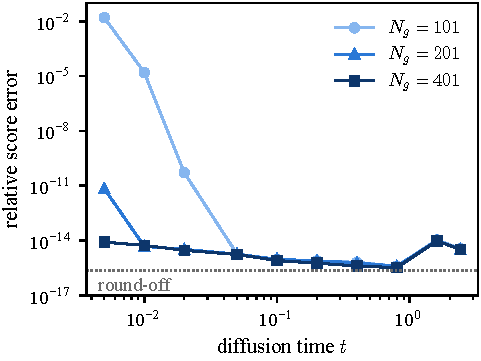
\includegraphics{fig_grid_gaussian}\hfill
  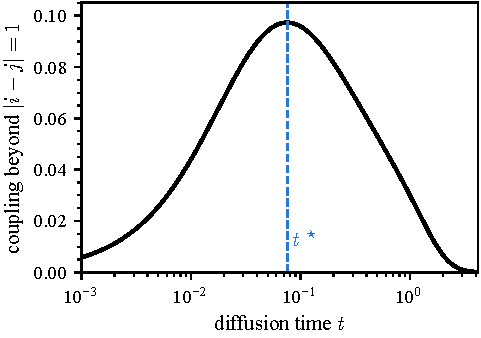
\includegraphics{fig_locality_curve}
  \caption{Left: grid BP against the exact score $-Q_tx$ on the Gaussian chain ($\alpha=0.8$) for three grid sizes;
  the dotted line is double-precision round-off. Right: coupling of $Q_t$ beyond nearest neighbours, relative to the
  nearest-neighbour coupling of $Q_0$, against $t$; it peaks at $t^\star$.}
  \label{fig:grid}
\end{figure}

\section{EM: M-steps}
\label{app:em}

\note{Closed forms: Gaussian AR(1) (posterior-weighted Yule--Walker), Laplace AR(1) (weighted median), mixture (ECM),
log-linear families (concave $Q$, gradient = observed minus expected), neural energy (autograd on $Q$, GEM: a few
Adam steps per iteration, step halved when $Q$ does not increase). Checkpoint ladder and selection rule.}

\begin{figure}[h]
  \centering
  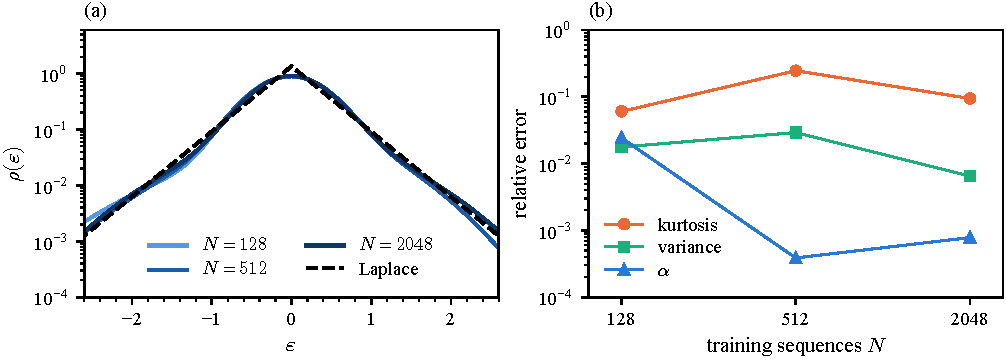
\includegraphics{fig_em_innovation}
  \caption{Mixture kernel ($C=8$). (a) Learned innovation law against the Laplace truth. (b) Relative error of
  $\alpha$, of the innovation variance and of its excess kurtosis against $N$, one fit per $N$.}
  \label{fig:em-innovation}
\end{figure}

\section{Sources of error}
\label{app:errors}

\note{J\'er\^ome: the error decomposition goes here. Grid (quadrature and truncation), kernel misspecification,
finite data, EM stopping. Thesis Ch.~7--8.}

\section{Network baselines}
\label{app:networks}

\note{Six architectures, parameter counts, hyperparameter screen, training recipe (DSM on clean sequences, Adam,
checkpoints at 500--32{,}000 steps, validation selection), the pairing with EM--BP on the same test sequences (E02a and
E03).}

\section{Allen--Cahn details}
\label{app:field}

\note{Cells (temperature, spacing, correlation), the family definitions (site energy, tilted spline, log-linear 2-D,
MDN, shift mixture), the networks, and the $M=128$ table.}

\begin{table}[h]
  \caption{As \cref{tab:field}, from $M=128$ training sequences.}
  \centering
  \small
  \begin{tabular}{@{}lcccc@{}}
    \toprule
    $\Theta$ & 0.3 & 0.5 & 1 & 2\\
    \midrule
    site energy          & 0.139 & 0.269 & 0.534 & 0.630\\
    tilted spline        & 0.218 & 0.454 & 1.110 & 1.478\\
    log-linear 2-D       & 0.385 & --    & 1.337 & --\\
    MDN                  & 0.468 & 0.900 & 1.724 & 2.457\\
    shift mixture        & 1.018 & 1.039 & 1.187 & 1.278\\
    best network         & 0.829 & 2.339 & 4.150 & 5.787\\
    \bottomrule
  \end{tabular}
  % src: ~/Code/Thesis/jerome-call-2026-10-29-slide15.md, M = 128 table
\end{table}


\end{document}
